%\section{Projection results}
\paragraph{Model-independent limits}
\label{sec:model_indep}
%
The model independent 
95\% confidence level (\CL) upper
limit on the cross sections for the ggH and bbH 
production modes, 
with the subsequent decays $\PH\to\tau\tau$,
are shown in Figs.~\ref{fig:model_indep} and Fig.~\ref{fig:model_indep2} for 
integrated luminosities of 300, 3000 and 6000\fbinv.
The 6000\fbinv limit is an approximation of the sensitivity with the complete HL-LHC 
dataset to be collected by the ATLAS and CMS experiments, corresponding to an integrated 
luminosity of 3000\fbinv each. The approximation assumes that the results of the 
two experiments are uncorrelated and that their sensitivity is similar. The first 
assumption is fulfilled to a high degree because the results are statistically limited; 
the validity of the second assumption is evident by comparing previous limits and 
projections. 
%
\begin{figure}[htbp]
\begin{center}
\subfloat[ggH]{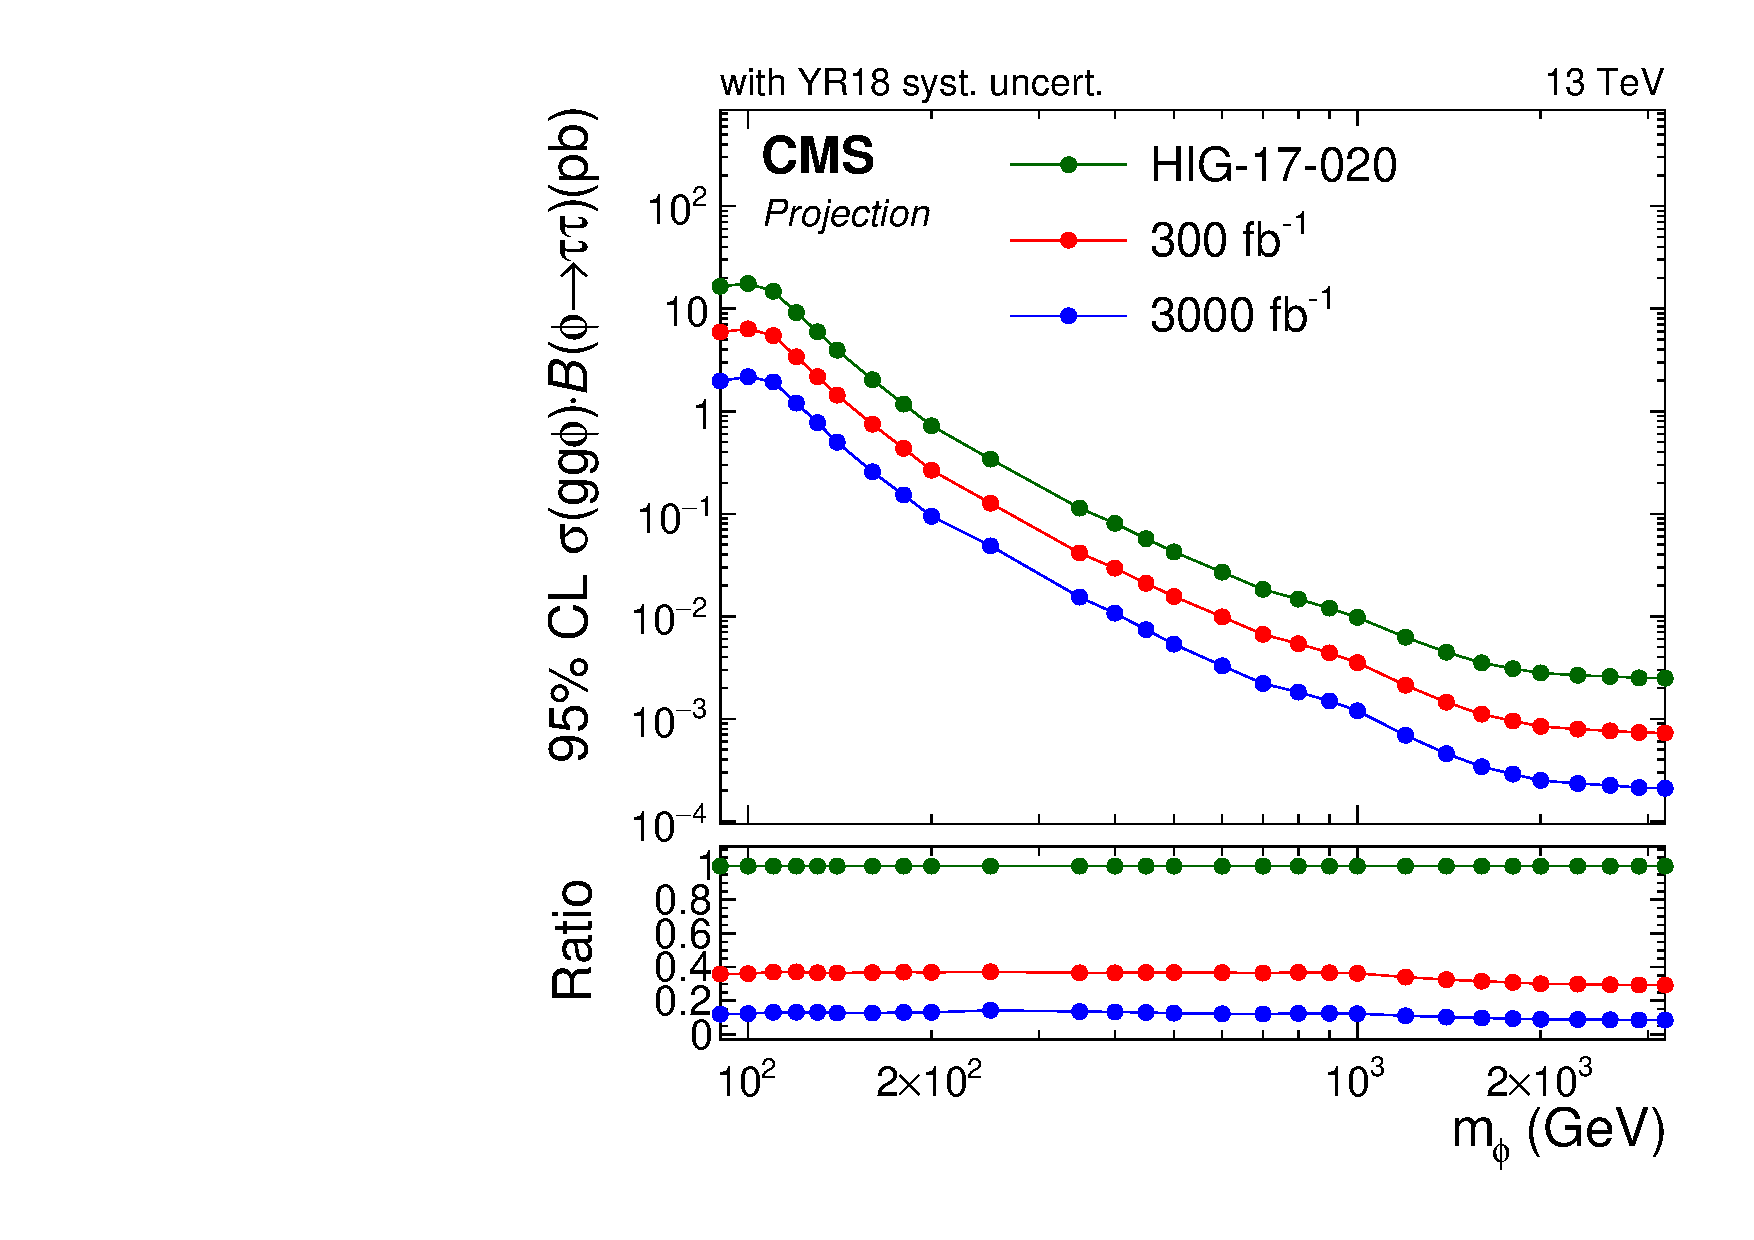
\includegraphics[width=0.45\textwidth]{\main/section9/cms_htt/figures/scen2_ggH_pas.pdf}}
\subfloat[bbH]{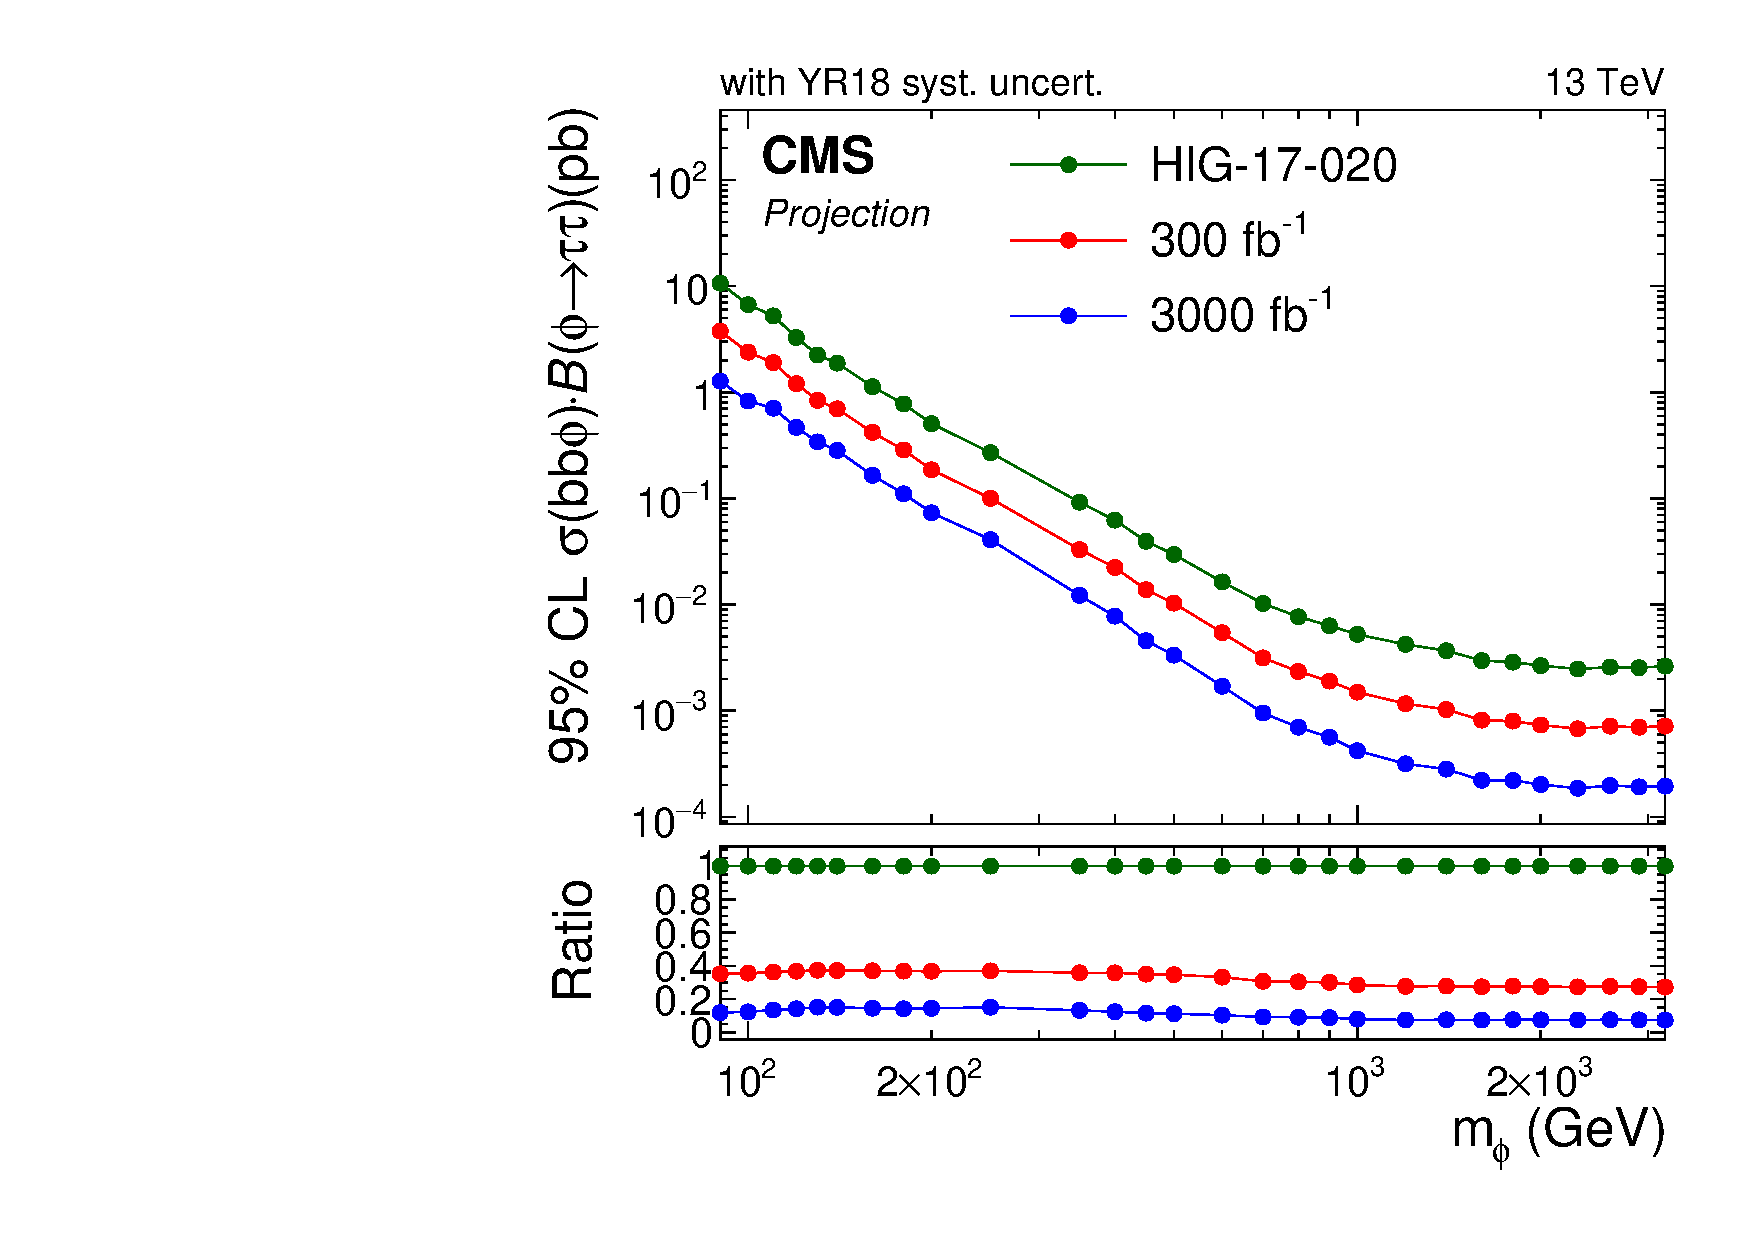
\includegraphics[width=0.45\textwidth]{\main/section9/cms_htt/figures/scen2_bbH_pas.pdf}}
\end{center}
\caption{Projection of expected model independent
  95\% CL upper limits based on 2016 CMS data~\cite{HIG-17-020} for 
ggH and bbH production with subsequent \htt decays, with YR18 systematic 
uncertainties. 
The limit shown for 6000\fbinv is an approximation of the 
sensitivity with the complete HL-LHC dataset to be collected by the ATLAS and 
CMS experiments, corresponding to an integrated luminosity of 3000\fbinv each.
The limits are compared to the CMS result using 2016 data~\cite{HIG-17-020}.}
\label{fig:model_indep}
\end{figure}

For both production modes, 
the improvement in the limits at high mass values
scales similarly to the square root of the integrated luminosity,
as expected from the increase in statistical precision.
The improvement at very low mass is almost entirely a consequence of reduced systematic uncertainties
and not the additional data in the signal region. 
The difference between the Run 2 and YR18 scenarios is mostly because of the treatment 
of two kinds of systematic uncertainty of a statistical nature: 
the uncertainty related to the number of simulated events 
and that related to the number 
of events in the data control regions.
%
\begin{figure}[htbp]
\begin{center}
\subfloat[ggH]{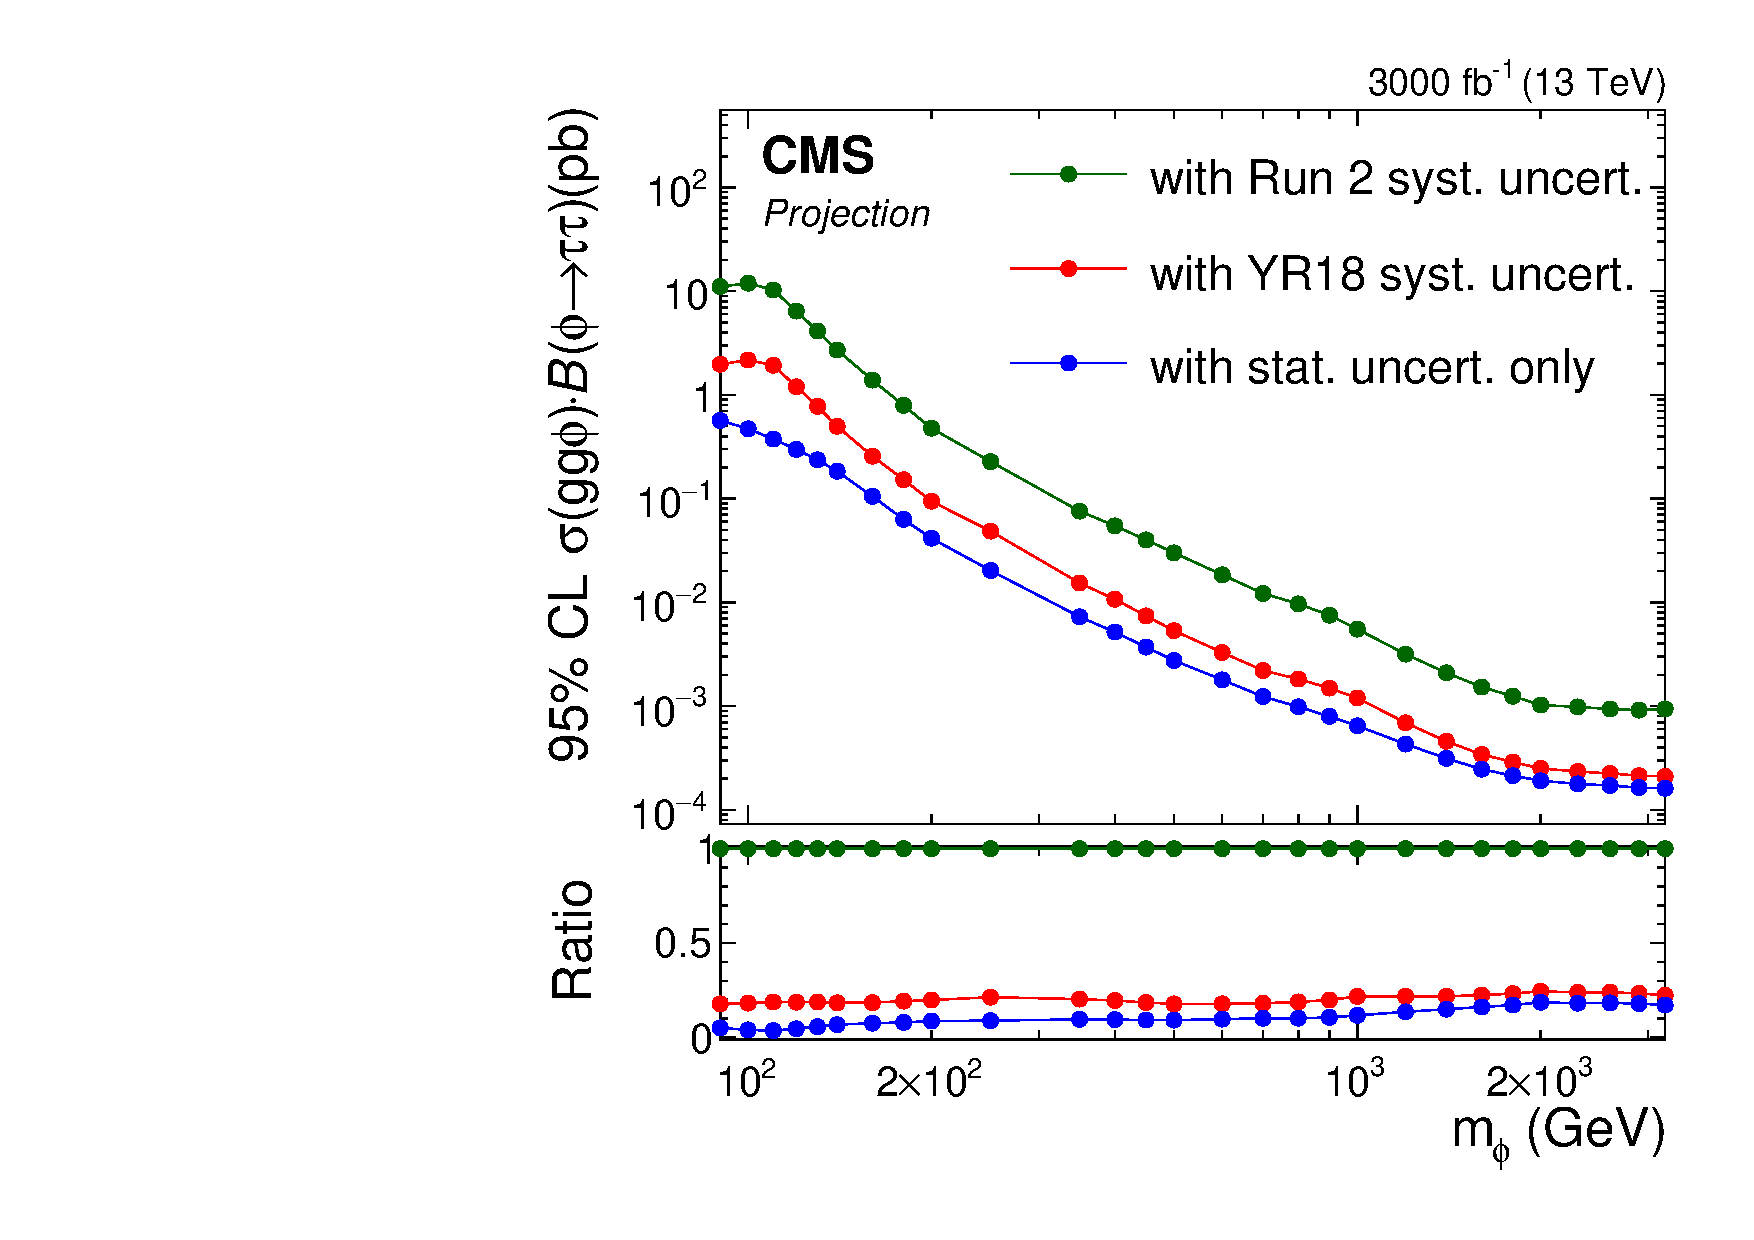
\includegraphics[width=0.45\textwidth]{\main/section9/cms_htt/figures/3000fb_ggH_pas.pdf}}
\subfloat[bbH]{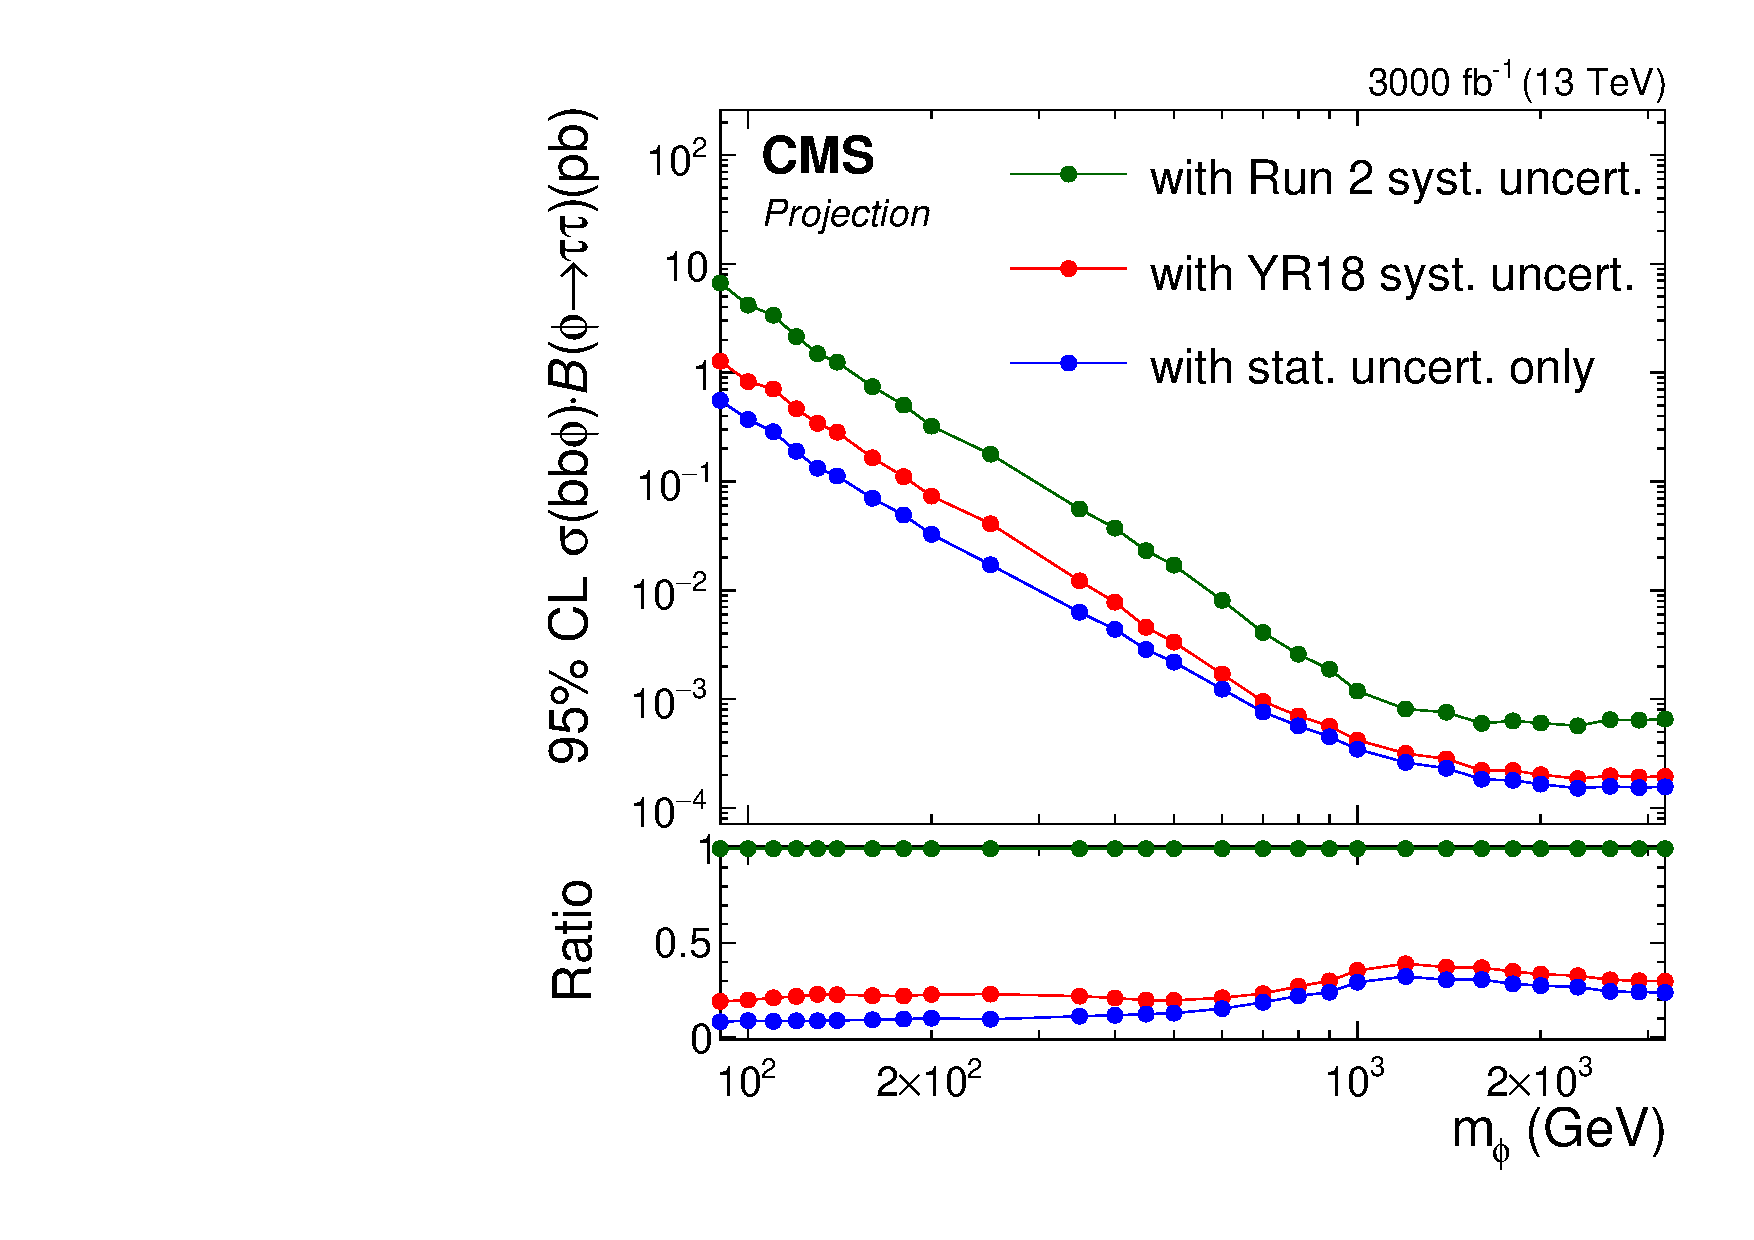
\includegraphics[width=0.45\textwidth]{\main/section9/cms_htt/figures/3000fb_bbH_pas.pdf}}
\end{center}
\caption{Projection of expected model-independent limits based on 2016 CMS data~\cite{HIG-17-020} 
for ggH and bbH production with subsequent \htt decays, comparing different 
scenarios for systematic uncertainties for an integrated luminosity of 3000\fbinv.}
\label{fig:model_indep2}
\end{figure}

\begin{figure}[htbp]
\begin{center}
\subfloat[ggH]{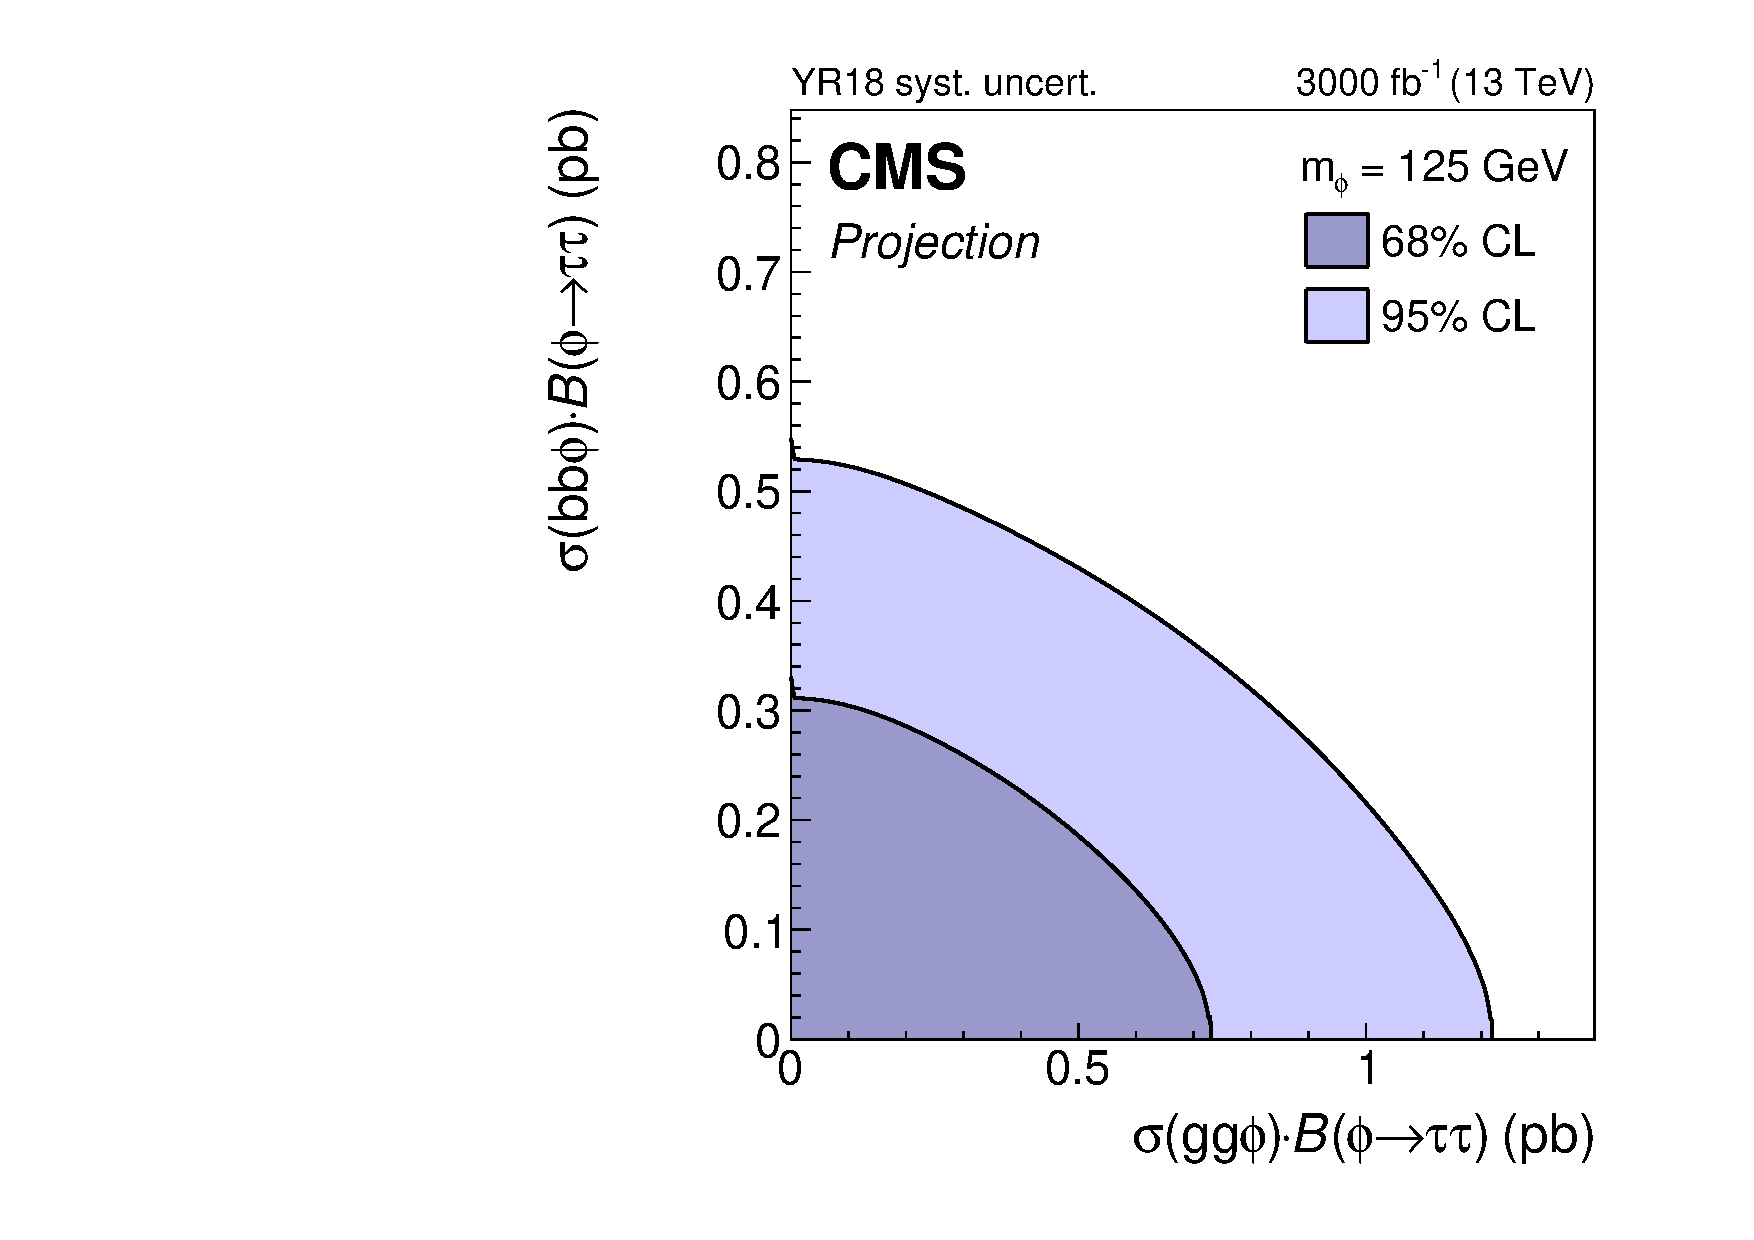
\includegraphics[width=0.45\textwidth]{\main/section9/cms_htt/figures/2D_limit_mH125.pdf}}
\subfloat[ggH]{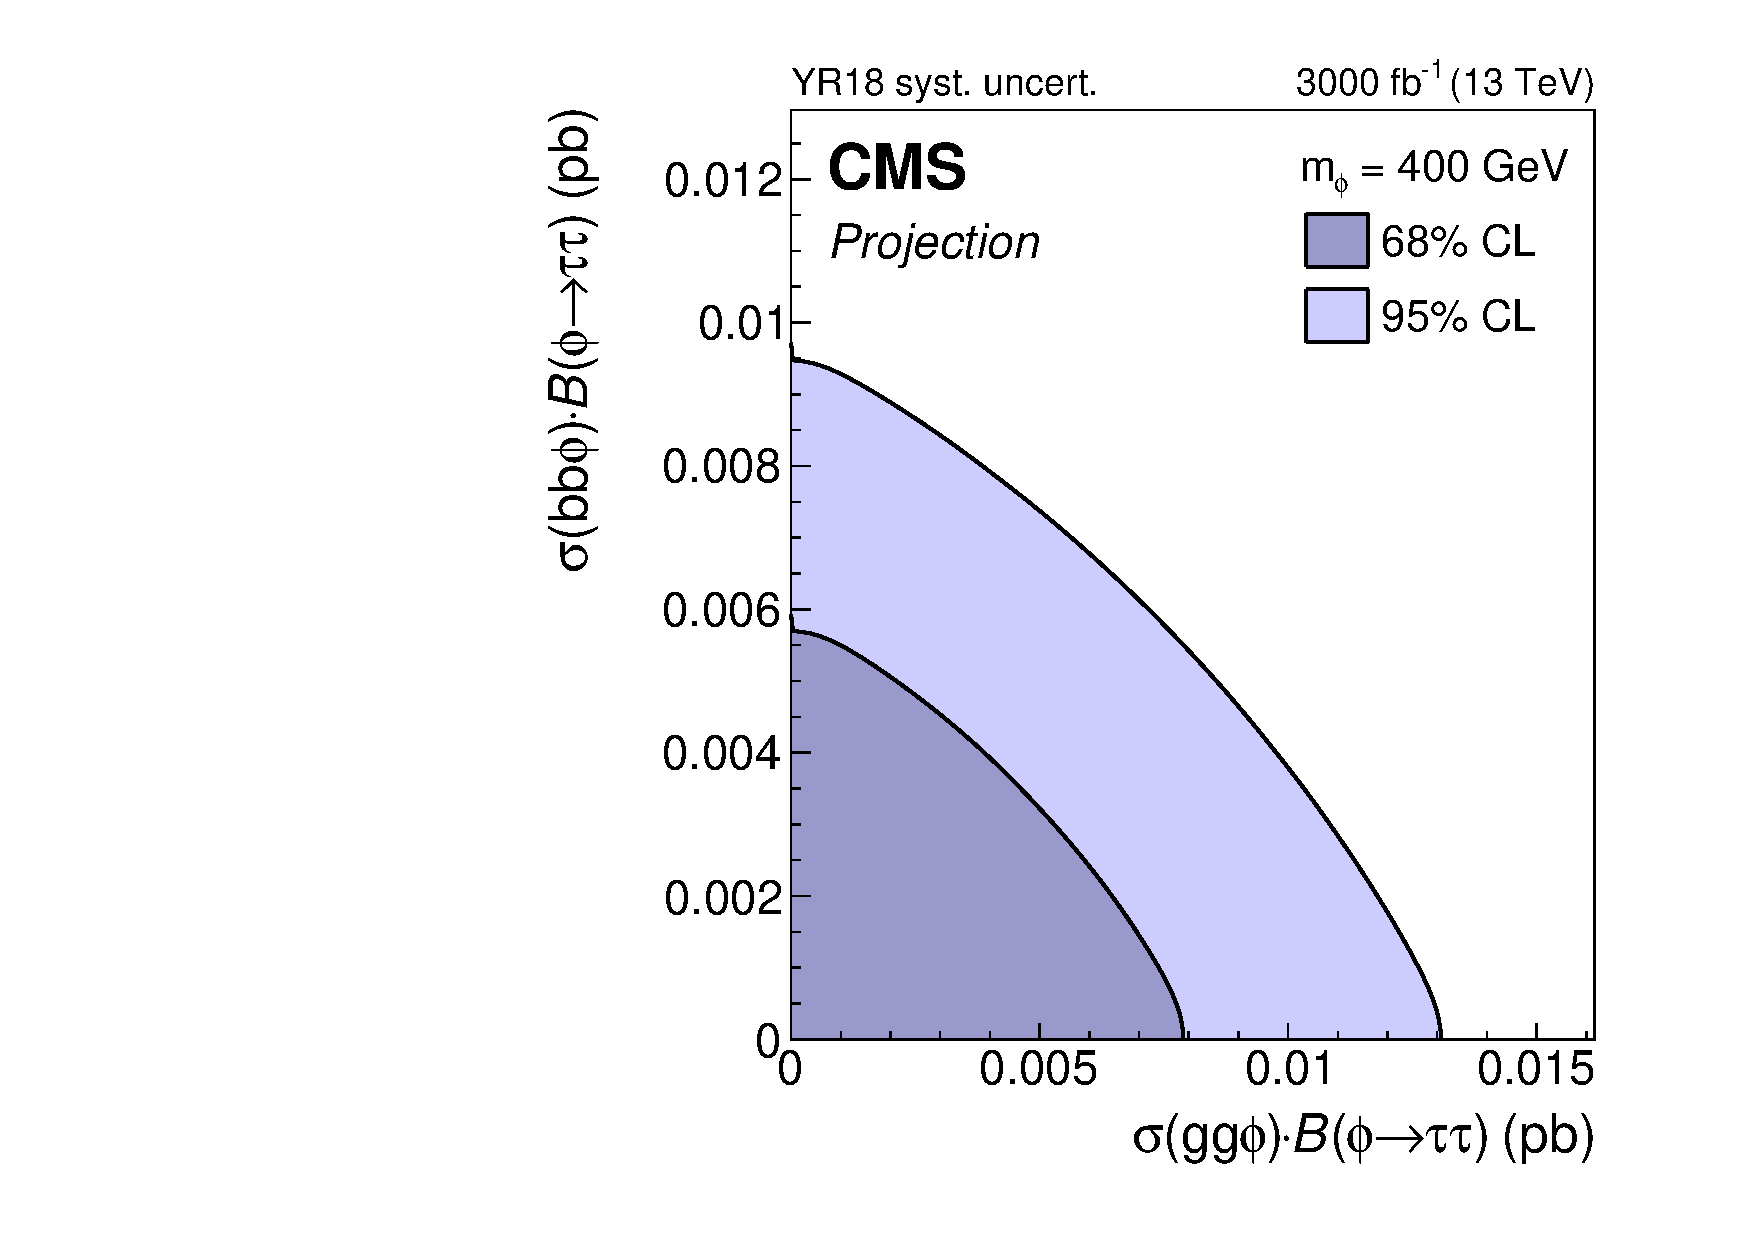
\includegraphics[width=0.45\textwidth]{\main/section9/cms_htt/figures/2D_limit_mH400.pdf}}\\
\subfloat[ggH]{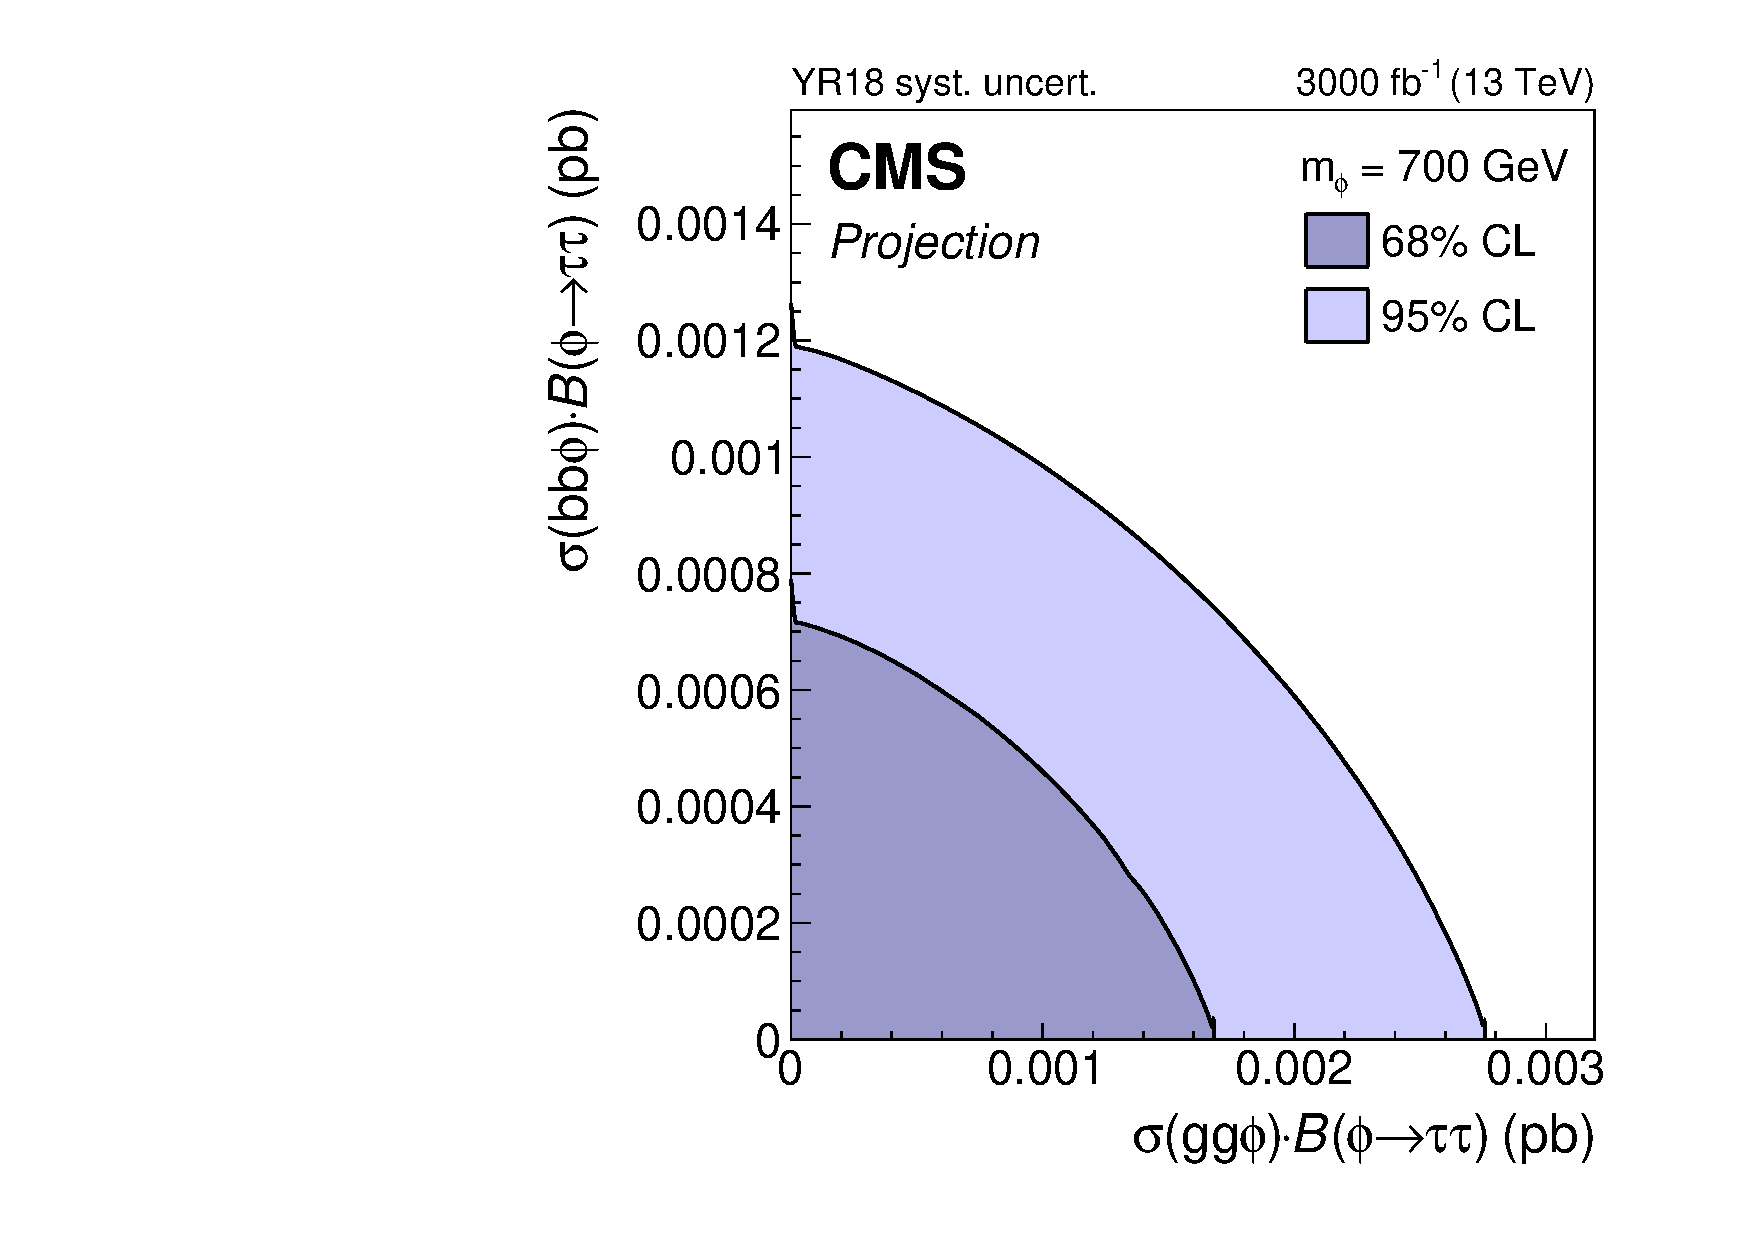
\includegraphics[width=0.45\textwidth]{\main/section9/cms_htt/figures/2D_limit_mH700.pdf}}
\subfloat[ggH]{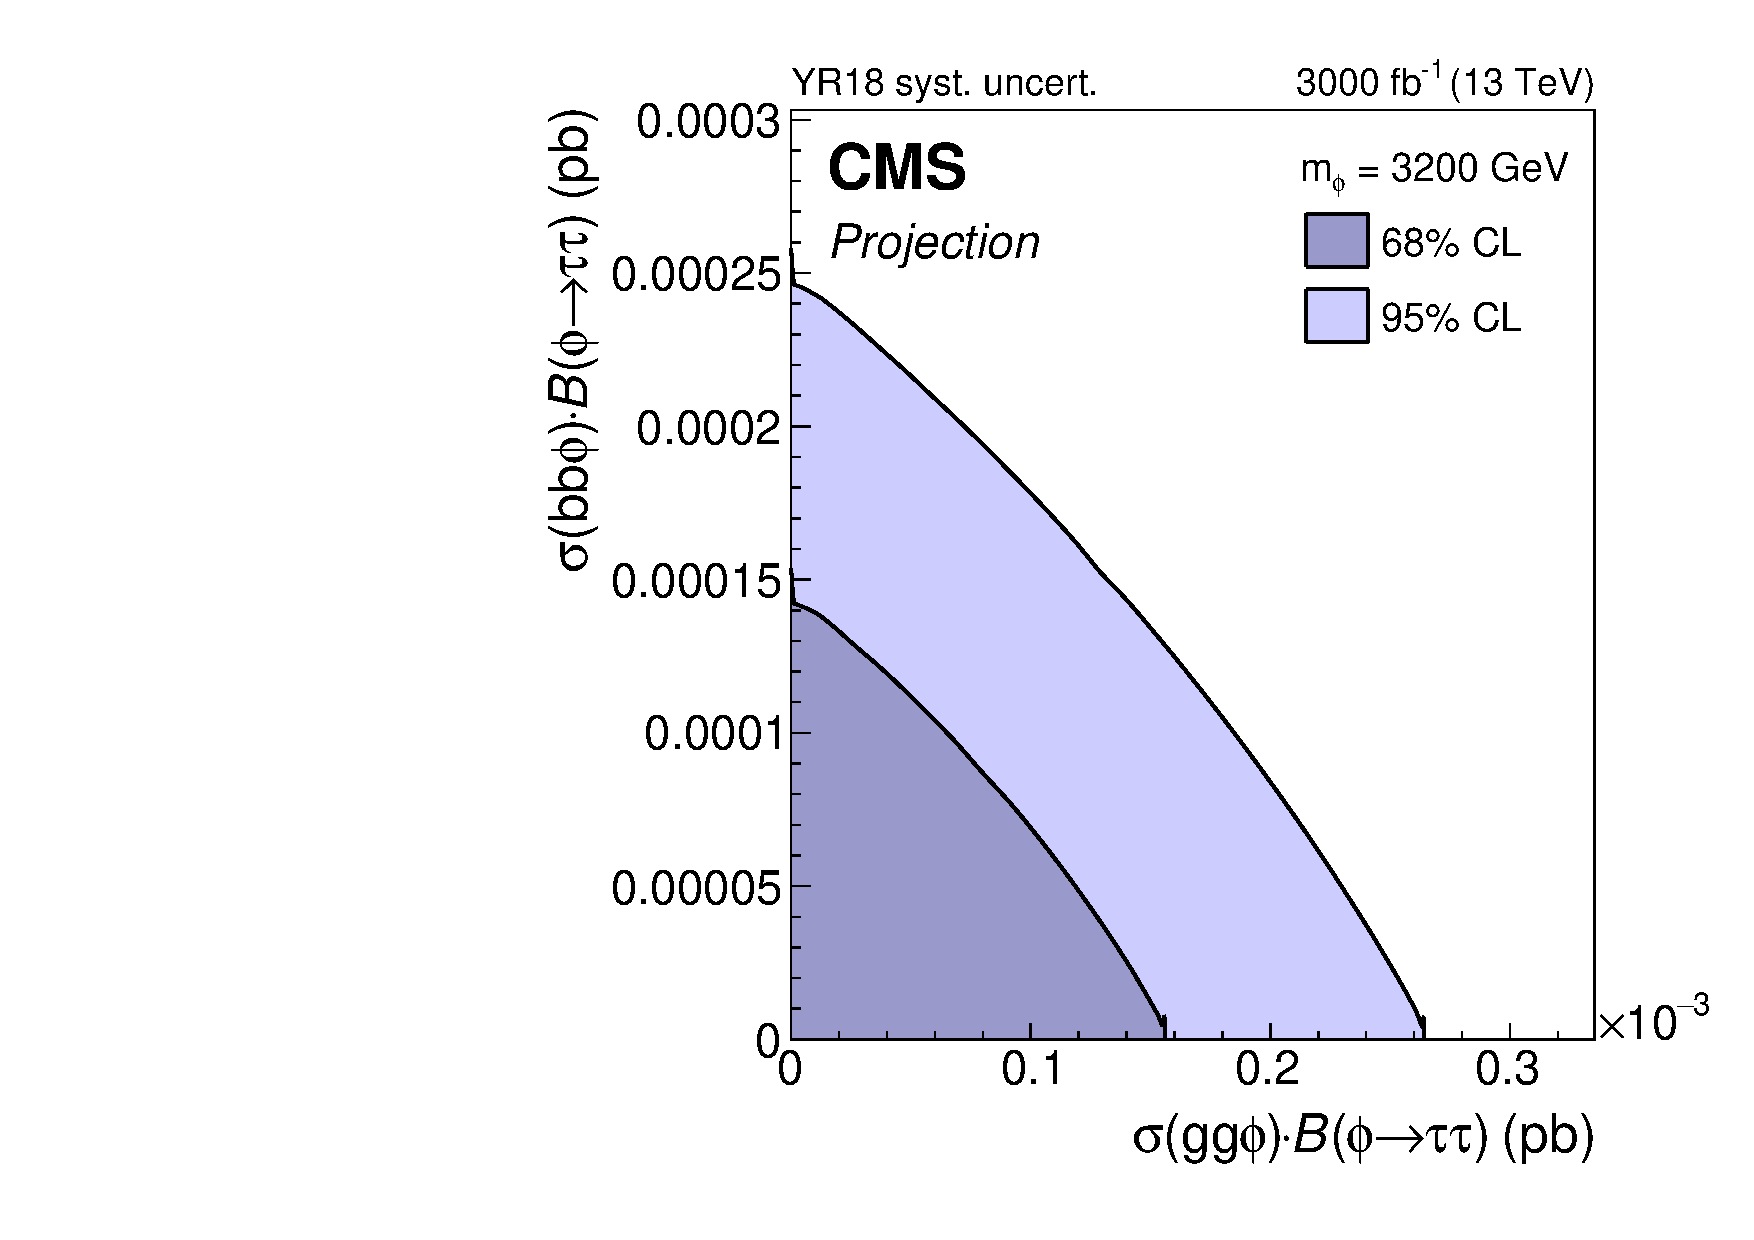
\includegraphics[width=0.45\textwidth]{\main/section9/cms_htt/figures/2D_limit_mH3200.pdf}}
\end{center}
\caption{Projection of expected model-independent limits based on 2016 CMS data~\cite{HIG-17-020} for a simultaneous fit to the ggH and bbH production cross sections with subsequent \htt decays, 
for an integrated luminosity of 3000\fbinv and with YR18 systematic uncertainties.}
\label{fig:model_indep2d}
\end{figure}